Následující část diplomové práce představuje implementaci nástroje pro automatickou správu Solaris Zones. V~úvodu
kapitoly je představen použitý programovací jazyk a~důvody pro jeho použití. Hlavní částí
je popis knihovny, modulu Solaris Zones a~klientské aplikace. Důraz je kladen na popis funkcionality jednotlivých 
částí aplikace a~jejich vzájemné komunikace.
\section{Programovací jazyk}
\label{chapter:implementation:language}
Prvním krokem  při implementaci bylo zvolení vhodného programovacího jazyka. Požadavky stanovené v~kapitole 
\ref{chapter:design:demands} vyžadují od zvoleného programovacího jazyka následující dvě podmínky:
\begin{itemize}
 \item operační systém Solaris,
 \item možnost tvorby grafického rozhraní.
\end{itemize}
Nástroj pro automatickou správu virtualizačního kontejneru Solaris Zones využívá
nástrojů na příkazové řádce a~zpracovává jejich výstup. Pro tento účel bylo vhodné zvolit interpretovaný
programovací jazyk, který umožnil jednoduše spustit nástroje a~následně snadno zpracovat jejich výstup. Na základě
výstupu se pak nástroj rozhodne o~dalším průběhu zpracování uživatelského příkazu. První podmínka není pro volbu jazyka
tolik omezující. Pro operační systém Solaris existuje implementace standardního kompilátoru \verb|gcc(1)|
pro jazyk C a~stejně tak implementace virtuálního stroje JVM pro jazyk Java. Většina interpretovaných jazyků
staví svůj překladač právě nad jedním z~těchto základních programovacích jazyků.

Z~výše uvedených důvodů bylo nutné při volbě jazyka dbát hlavně na~dostupnost grafických knihoven pro operační systém
Solaris. \verb|Shell| je standardním skriptovacím jazykem pro většinu operačních systému typu UNIX. Tento program
interpretuje uživatelské příkazy na příkazové řádce a~následně je provádí. Tato volba by splňovala podmínku platformy,
ale těžko by se s~pomocí tohoto jazyka vytvářelo grafické uživatelské rozhraní. Z~tohoto důvodu byl zvolen programovací
jazyk Ruby \cite{ruby}, který umožnil splnit obě stanovené podmínky.
\subsection{Ruby}
\label{chapter:implementation:language:ruby}
Ruby je objektově orientovaný programovací jazyk, který má mnoho možností využití. Jedním ze scénářů využití může být
právě spouštění příkazů na~příkazové řádce a~tvorba uživatelského rozhraní. Objektová povaha tohoto jazyka umožňuje
programátorovi využívat všech výhod objektově orientovaného programování. Podle dokumentu \cite{ruby:implementation}
existuje několik implementací interpretu jazyka Ruby, z~nichž nejpoužívanější jsou YARV \cite{ruby:implementation:yarv} 
a~JRuby \cite{ruby:implementation:jruby}. Obě tyto implementace jsou dostupné i pro operační systém Solaris.

Pokud chce programátor využívat grafické rozhraní pomocí programovacího jazyka Ruby, je nutné, aby byly v~systému
nainstalované potřebné grafické knihovny. Standardní knihovny pro programovací jazyk Ruby však nejsou na~operačním
systému Solaris podporované. Z~toho důvodu bylo nutné využít grafické rozhraní, které nabízí implementace JRuby.
Tato implementace je postavená nad virtuálním strojem JVM a~může využívat grafické knihovny v~něm implementované.
Navrhovaný nástroj pro automatickou správu virtualizačního kontejneru Solaris Zones tedy využívá programovacího
jazyka Ruby. Pokud bude chtít uživatel nástroje využívat grafického rozhraní, musí nástroj spouštět pomocí
interpretu JRuby. Zbytek nástroje je nezávislý na použitém interpretu programovacího jazyka Ruby.
\section{Knihovna}
\label{chapter:implementation:library}
Hlavním centrálním prvkem implementace je knihovna, která zprostředkovává komunikaci mezi implementovanými moduly
a~klientskými aplikacemi. Knihovna je navržená tak, aby se v~budoucnosti dala lehce rozšířit o~další moduly, které budou
poskytovat funkce pro správu jiných virtualizačních technologií. Jedním z~takových rozšíření by mohl být například modul
pro podporu virtualizační technologie Oracle VirtualBox. Výsledná implementace obsahuje pouze modul pro podporu automatické
správy virtualizačního kontejneru Solaris Zones, který bude popsán v~kapitole \ref{chapter:implementation:szones}.

Knihovna poskytuje hlavní rozhraní, pomocí kterého může klient využívat funkcí jednotlivých modulů. Jednotlivé
moduly tedy slouží jako hlavní zdroj funkcionality pro knihovnu.

Mimo zprostředkovávání komunikace mezi moduly a~klientem slouží kni\-ho\-vna k~validaci šablon, které mají specifikovat
konkrétní virtuální stroj. V~případě šablon knihovna funguje jako vstupní bod, který umí šablonu načíst a~provést
prvotní validaci. Spouštění těchto operací a~jejich výsledky knihovna zprostředkovává klientovi.

Jelikož moduly mohou implementovat různé typy operací pomocí různých technologií, je nutné ponechat vývojářům velkou volnost
v~možnostech jejich implementace. Pro účel zajištění jednotné komunikace s~moduly je nutné, aby každý implementovaný modul
splňoval určité rozhraní. Toto rozhraní zajistí, aby všechny moduly mohly jednotně komunikovat s~knihovnou a~také, aby knihovna
mohla zprostředkovávat jejich funkce klientovi.

Poslední funkcí knihovny je udržování hlavní konfigurace. V~této konfiguraci je například uchováván seznam implementovaných
modulů, kořenový adresář knihovny nebo například jméno knihovny. Klientská aplikace má možnost tuto konfiguraci změnit
a~docílit tak jiného chování knihovny.
\subsection{Rozhraní modulu}
\label{chapter:implementation:library:interface}
Povinné rozhraní modulu slouží především ke komunikaci mezi knihovnou a~samotným modulem. Funkcionalitu, kterou modul
musí poskytovat, je možné shrnout do následujících bodů:
\begin{itemize}
 \item inicializační rutina,
 \item rozhraní poskytované klientům,
 \item funkce pro validaci šablon.
\end{itemize}
Prvním požadavkem na rozhraní modulu je existence inicializační rutiny. Pomocí této rutiny je do modulu předána hlavní
konfigurace knihovny, která umožňuje modulu zjistit kořenový adresář aplikace a~další parametry. Hlavním smyslem
této rutiny je inicializace daného modulu. Hlavní knihovna v~rámci inicializační smyčky spustí tuto rutinu pro každý
registrovaný modul. Uvnitř této rutiny může modul provádět inicializaci vlastních datových struktur nebo vytvoření potřebné
adresářové struktury. Dále může modul využít hlavní konfiguraci knihovny k~doplnění vlastní lokální konfigurace. Tímto způsobem
je zajištěno, že všechny registrované moduly knihovny obdrží globální konfiguraci a~dojde k~jejich inicializaci.

Další nutnou částí rozhraní modulu jsou funkce, které mají být poskytovány klientovi. K~tomuto účelu musí modul poskytovat
třídu, která bude tyto funkce implementovat nebo je bude pouze zprostředkovávat pomocí jiných tříd modulu. Tato třída je tedy
hlavním funkčním rozhraním modulu, které klientské aplikace mohou využívat. V~rámci inicializace celé knihovny dojde nejprve
k~inicializaci jednotlivých modulů. Po této akci knihovna provede registraci těchto tříd a~v~udržuje si jejich seznam.

Posledním požadavkem na rozhraní modulu je existence funkcí pro validaci šablon. Tyto funkce musí umožňovat validovat šablony,
které se týkají konkrétního modulu knihovny. Modul, který podporuje správu virtualizačního kontejneru Solaris Zones, musí poskytovat
funkce pro validaci šablon specifikující neglobální zóny.

Vlastní implementace modulu není nijak jinak omezena. Jediným logickým omezením je fakt, že tento modul musí být napsaný
v~programovacím jazyku Ruby. Pokud modul splní výše zmíněné požadavky, může být jednoduše registrován do knihovny a~klientské
aplikace ho můžou bezprostředně po~inicializaci knihovny využívat. Na obrázku \ref{figure:module:interface} je názorně zobrazeno, 
jakým způsobem knihovna využívá rozhraní modulu a~jakým způsobem je modul poskytován klientské aplikaci.
\begin{figure}[ht]
    \centering    
    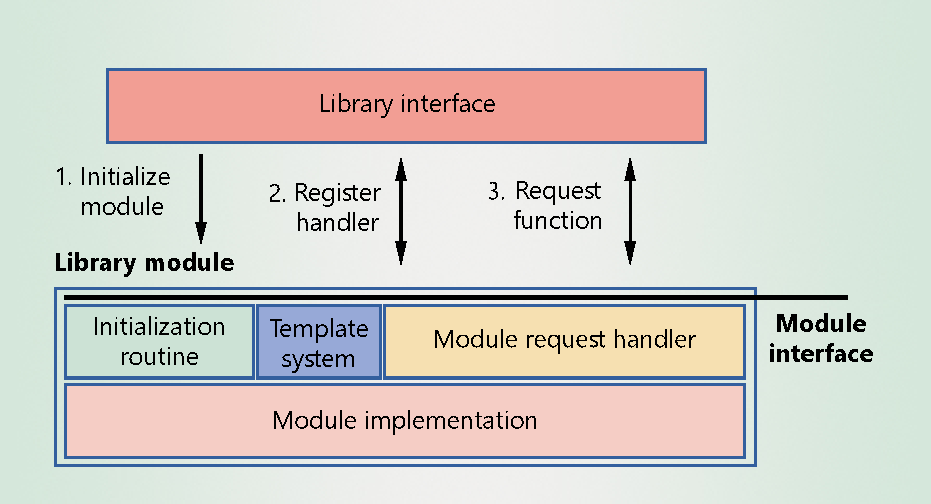
\includegraphics[scale=0.7]{assets/pdfs/module_interface.pdf}
    \caption{Rozhraní modulu}
    \label{figure:module:interface}
\end{figure}
\subsection{Přesměrování požadavků}
\label{chapter:implementation:library:routing}
Mimo inicializace modulů je hlavní funkcí knihovny přesměrovávat požadavky klientských aplikací na funkční rozhraní 
implementovaných modulů. K~tomuto účelu obsahuje knihovna hlavní třídu, která virtuálně reprezentuje rozhraní všech modulů
knihovny. Tato třída se nazývá hlavní rozhraní. Jak již bylo zmíněno,
knihovna si udržuje odkazy na hlavní třídy modulů, které reprezentují jejich funkční rozhraní.

V~okamžiku, kdy klientská aplikace vznese požadavek na zavolání konkrétní funkce, knihovna za běhu zjistí jakému modulu daná
funkce přísluší a~vyvolá ji. Pokud neexistuje žádný modul, který umí danou funkci provést, dojde k~vyvolání výjimky a~aplikace
se ukončí. Díky tomuto chování může dojít ke kolizi jmen funkcí. V~takovém případě by knihovna použila takovou funkci, kterou
by našla jako první v~pořadí. Z~tohoto důvodu je nutné se vyvarovat opakování jmen funkcí a~nejlépe používat pro funkce určitého
modulu prefix, který daný modul jasně identifikuje, například jeho jméno.

Toto směrování za běhu aplikace je umožněno díky programovacímu jazyku Ruby a~jeho možnosti dynamického volání funkcí za běhu
programu. Směrování požadavků ke konkrétním modulům knihovny je demonstrováno na obrázku \ref{figure:module:interface}.
\subsection{Generická šablona}
\label{chapter:implementation:library:generic}
Poslední funkcí knihovny je definice generické šablony, která má za~úkol specifikovat virtuální stroj. Hlavním úkolem
generické šablony je specifikovat typ virtuálního stroje. Tento atribut určuje, který modul knihovny je zodpovědný
za zpracování a~validaci. Generická šablona by dále měla obsahovat jméno, které bude nějakým způsobem vystihovat a~popisovat
specifikovaný virtuální stroj. Knihovna tedy zajišťuje validaci těchto dvou atributů a~v~případě úspěchu předá
šablonu zodpovědnému modulu.

Knihovna poskytuje klientským aplikacím funkce pro načítání a~validaci šablon. V~případě úspěšného načtení šablony
knihovna vrátí objekt, který je možné použít v~rámci konkrétního modulu. Validace šablony je prováděna ve~dvou
krocích. Knihovna nejprve zjistí, zdali daná šablona obsahuje atribut jména a~typu. Podle typu šablony se knihovna rozhodne
jakému modulu ji předá na druhý krok validace.
\subsubsection{Struktura šablony}
\label{chapter:implementation:library:generic:structure}
Aby mohla být šablona opakovaně používána pro tvorbu virtuálních strojů, musí být perzistentně uložena v~souborovém systému.
Pro tento účel je použitý datový formát JSON \cite{json}, který slouží pro reprezentaci šablony. Hlavním důvodem využití tohoto
formátu je relativně dobrá uživatelská čitelnost a~především snadné zpracování pomocí programovacího jazyka Ruby. Uživatel
může pro konstrukci šablony použít jednoduchý textový editor nebo grafický editor, který je součástí uživatelského rozhraní
klientské aplikace. 

Struktura šablony se skládá ze dvou částí. První částí je název a~definice typu šablony. Tato hlavička určuje
způsob zacházení s~danou šablonou. V~ukázce kódu \ref{code:generic_template} je naznačeno, jakým způsobem by mohla taková šablona vypadat.
Atribut \textit{type} určuje o~jaký typ virtuálního stroje se jedná a~k~jakému modulu knihovny přísluší. Druhou povinnou položkou
v~šabloně je atribut \textit{name}, který má za~úkol popsat funkcionalitu virtuálního stroje. Tečky v~ukázce
\ref{code:generic_template} reprezentují atributy specifické pro konkrétní typ šablony. Tyto atributy jsou z~ukázky vynechány.
\begin{listing}[ht]
  \caption{Demonstrace generické šablony}
  \begin{minted}{JSON}
{
  "name": "template_webserver",
  "type": "szones",
  ...
}   
  \end{minted} 
  \label{code:generic_template}
\end{listing}
\subsubsection{Validace šablony}
\label{chapter:implementation:library:generic:validation}
Šablona musí poskytovat validní definici virtuálního stroje, aby z~ní bylo možné konkrétní virtuální stroj zkonstruovat.
Pro tento účel je nutné zavést validaci šablon a~jejich atributů. Jelikož je pro ukládání šablon použit datový formát JSON,
je pro validaci šablony použité tvz. JSON schéma definované ve~specifikaci \cite{json:schema}. Tento dokument je opět ve formátu
JSON, ale neslouží pro ukládání dat. Jeho funkcí je definovat formát jiného dokumentu JSON. Pomocí tohoto schématu
je možné specifikovat atributy a~typy jejich hodnot, které má konkrétní typ dokumentu obsahovat.

Tento nástroj umožňuje definovat, jaké atributy může konkrétní typ virtuálního stroje mít. Pokud uživatel sestrojí
nevalidní šablonu virtuálního stroje, knihovna skrze validaci JSON dokumentu pozná, že se jedná o~neplatnou konfiguraci. Knihovna
implementuje základní schéma, které slouží pro základní validaci šablon. Jak je vidět v~ukázce \ref{code:generic_tmplate:validation},
toto schéma vyžaduje, aby v~dokumentu byly přítomné atributy \textit{name} a~\textit{type}. Moduly aplikace musí implementovat
podrobnější schéma, které má definovat konkrétní typ virtuálního stroje.

Aby bylo možné v~programovacím jazyku Ruby validovat JSON dokumenty, je nutné použít knihovnu, která bude implementovat
JSON schéma. Pro tento účel aplikace využívá volně dostupné řešení \textit{json-schema} \cite{json:schema:ruby}, které implementuje
funkce validace dokumentů typu JSON pomocí schémat.
\begin{listing}[ht]
  \caption{Schéma generické šablony}
  \begin{minted}{JSON}
{
  {
  "title": "general-vm-template",
  "description": "Used for general template distinction",
  "type": "object",
  "properties": {
    "name": {
      "type": "string",
      "description": "Name of the vm template"
    },
    "type": {
      "enum": [ "szones", "vbox" ],
      "description": "Type of the vm template"
    }

  },
  "required": [ "name", "type" ],
  "additionalProperties": true
}  
  \end{minted} 
  \label{code:generic_tmplate:validation}
\end{listing}
\section{Modul Solaris Zones}
\label{chapter:implementation:szones}
Modul Solaris Zones je hlavním stavebním kamenem celé implementace výsledného nástroje. Tento modul je zařazen do knihovny
popsané v~kapitole \ref{chapter:implementation:library} a~mimo jiné poskytuje základní rutiny pro správu virtualizačního
kontejneru Solaris Zones. Aby mohl být tento modul využíván knihovnou, musí implementovat rozhraní definované v~kapitole \ref{chapter:implementation:library:interface}.
Takto podmínka zahrnuje především implementaci tříd pro zpracovávání šablon virtuálních strojů. V~rámci tohoto modulu
se jedná o~šablony, které specifikují vlastnosti neglobálních zón. 

Funkcionalita modulu je rozdělena do několika vrstev, které se vzájemně využívají. Názvy jednotlivých vrstev jsou následující:
\begin{itemize}
 \item management šablon,
 \item nástroje pro správu Solaris Zones,
 \item administrátorské rutiny,
 \item funkční rozhraní modulu.
\end{itemize}
Architekturu vrstev modulu je možné pozorovat na obrázku \ref{image:implemetation:szones}. V~následujících kapitolách
bude podrobně popsána funkce jednotlivých vrstev a~jejich vzájemná interakce.
\begin{figure}[ht]
    \centering
    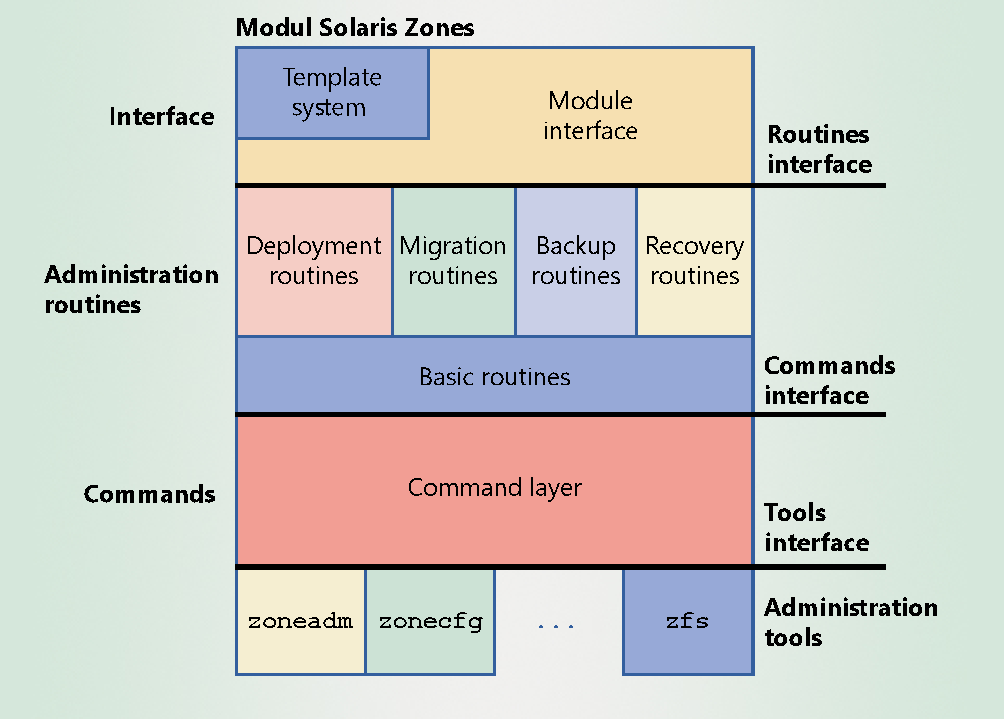
\includegraphics[scale=0.7]{assets/pdfs/module.pdf}
    \caption{Architektura modulu Solaris Zones}
    \label{image:implemetation:szones}
\end{figure}
\subsection{Šablona Solaris Zones}
\label{chapter:implementation:szones:template}
Nástroje pro správu Solaris Zones neposkytují možnost vytvářet zóny pomocí jednoho předpisu. Jak bylo popsáno v~kapitole
\ref{chapter:zones}, k~úspěšnému vytvoření neglobální zóny se využívají tři soubory. Prvním a~povinným parametrem instalace zóny
je její konfigurace. Není podmínkou, aby konfigurace zóny byla v~podobě souboru, ale pro automatizaci tohoto procesu je to výhodné.
Dále je nutné instalátoru předat definici softwarových balíků, které má nainstalovat. Posledním nepovinným parametrem instalace
je konfigurace systémových služeb. Aby bylo možné nainstalovat zónu pomocí jednoho souboru, musí tato šablona kombinovat
vlastnosti výše zmíněných souborů. 

Kostra šablony pro neglobální zónu je demonstrována v~ukázce kódu \ref{code:szones_template}. Z~ukázky je patrné, že šablona obsahuje
tři sekce, které korespondují s~jednotlivými soubory vyžadovanými při instalaci. Z~ukázky jsou vynechány konkrétní atributy zón.
Modul implementuje JSON schéma, které využívá pro validaci šablony a~pro mechanizmy jejího zpracování. Úkolem modulu při zpracování
šablony je reprodukce souborů s~konfigurací, manifestem a~systémovým profilem. Tyto soubory nástroj využívá pro instalaci 
neglobální zóny s~parametry, které jsou v~dané šabloně specifikovány.
\begin{listing}[ht]
  \caption{Kostra šablony pro neglobální zóny}
  \begin{minted}{JSON}
{  
  "name": "template_webserver",
  "type": "szones",
  "configuration": {...},
  "manifest": {
    "packages": [...]
   },
   "profile": {...} 
}
  \end{minted} 
  \label{code:szones_template}
\end{listing}
Pokud modul zpracovává rutinu, která využívá šablonu, je v~prvním kroku šablona rozdělena do třech zmíněných částí.
V~následujícím kroku jsou tyto části převedeny do vnitřní reprezentace a~následně zpracovány.
\subsubsection{Zpracování konfigurace}
\label{chapter:implementation:szones:template:configuration}
Konfigurační sekce šablony se skládá z~definice globálních atributů zóny popsaných v~kapitole \ref{chapter:zones:configuration:global_attributes}
a~z~definice zdrojů zóny, které jsou popsané v~kapitole~\ref{chapter:zones:configuration:resources}. Jednoduché globální atributy
jsou v~šabloně specifikovány přímo pomocí jejich jména a~hodnoty. Pro globální atribut typu zóny může definice vypadat 
následovně \mintinline{JSON}{{"brand": "solaris"}}.

Dále tato sekce šablony obsahuje definici zdrojů zóny, které mají složitější strukturu a~obsahují několik atributů. Z~tohoto
důvodu šablona obsahuje speciální atribut \mintinline{JSON}{{"resources": []}}, který je typu pole a~obsahuje definici
všech zdrojů zóny. V~rámci jednotlivého zdroje je použita stejná technika definice atributu jako ve výše zmíněném případě
globálních atributů.

Cílem zpracování této části šablony je vygenerovat soubor s~konfigurací, který má přesně definovanou syntaxi. Pomocí načtené
šablony uchované v~asociativním poli jsou globální atributy přetransformované do podoby, kterou vyžaduje nástroj \verb|zonecfg(1)|.
V~případě zdrojů je proveden stejný postup s~tím rozdílem, že se před každý zdroj přidá příkaz \verb|add| a~jeho definice
se ukončí příkazem \verb|end|. Takto přetransformovaná konfigurace je připravena k~použití v~nástroji \verb|zonecfg(1)|.
\subsubsection{Zpracování manifestu}
\label{chapter:implementation:szones:template:manifest}
V~rámci sekce šablony s~názvem \texttt{manifest} může uživatel specifikovat softwarové balíky, které má zóna obsahovat.
Pro tento účel obsahuje tato část šablony atribut \mintinline{JSON}{{"packages": []}}, který je typu pole. Hodnotou každého
prvku pole je obyčejný textový řetězec, který obsahuje jméno softwarového balíku. V~tomto poli může uživatel specifikovat libovolné
množství balíků. 

Cílem zpracování této sekce šablony je vytvořit manifest popsaný v~kapitole \ref{chapter:zones:instalation:repozitory:manifest}.
K~tomuto účelu si modul drží kopii tohoto souboru, která nese název \textit{manifest\_template.xml} a~nachází se v~kořenovém 
adresáři aplikace ve~složce \textit{szones/manifest}. Při zpracovávání manifestu jsou jednotlivé balíky načteny ze šablony
a~ve správném formátu vloženy do kopie tohoto souboru. Výsledný soubor je možné použít pro instalaci zóny.
\subsubsection{Zpracování systémového profilu}
\label{chapter:implementation:szones:template:profile}
Poslední částí zpracovávání šablony je transformace systémového profilu. Tato sekce slouží k~nastavení systémových služeb
neglobální zóny a~má stejnou strukturu jako sekce s~konfigurací zóny. Na rozdíl od způsobu zpracování konfigurační sekce je
však v~tomto případě vyžadován jiný výstup. Cílem této transformace má být soubor v~XML formátu popsaný v~kapitole \ref{chapter:zones:instalation:profile}.

Pro každou službu existuje korespondující soubor obsahující potřebnou část výsledného XML souboru. Tyto soubory jsou
uloženy v~kořenovém adresáři aplikace ve složce \textit{szones/profile}. V~průběhu zpracovávání šablony jsou jednotlivé soubory
načítány a~vyplňovány hodnotami ze šablony. Tímto způsobem se zkonstruuje celý soubor, který může být předán instalátoru.
\subsection{Nástroje}
\label{chapter:implementation:szones:commands}
Základním stavebním kamenem modulu je vrstva, která zajišťuje vykonávání potřebných příkazů na příkazové řádce.
Tato vrstva poskytuje vyšším vrstvám modulu možnost vykonávání základní administračních příkazů pro správu Solaris Zones
a~souborového systému ZFS.

Pro účel vykonávání příkazů tato vrstva implementuje třídu, která umožňuje provádění příkazů jak na lokálním tak i
na vzdáleném serveru. Tato třída nevykonává daný příkaz okamžitě, ale umožňuje vyšším vrstvám aplikace vykonání odložit.
Tento požadavek je na třídu kladen zejména z~důvodu efektivity využívání vytvořených SSH spojení. Dále třída umožňuje
definovat automatické chování v~případě chyby prováděného příkazu. Pro každý nástroj využívaný aplikací je definována sada
pravidel, které jsou uplatňovány na chybové výstupy nástrojů a~následně jsou vyvolávány příslušné výjimky. Vyšší vrstvy
aplikace musí tyto výjimky odchytávat a~adekvátně na ně reagovat.

Pomocí výše zmíněné třídy tato vrstva modulu umožňuje volat jednotlivé nástroje s~požadovanými parametry a~argumenty.
Například umožňuje spouštět nástroj \verb|zonecfg(1)| se jménem konfigurované zóny a~cestou k~souboru s~konfigurací. Vyšším
vrstvám je poskytnutý standardní výstup a~standardní chybový výstup daného nástroje.
\subsection{Administrátorské rutiny}
\label{chapter:implementation:szones:routines}
Hlavní částí modulu je vrstva tříd, které implementují požadované rutiny pro~správu Solaris Zones. Rutiny využívají
nástrojů implementovaných v~nižší vrstvě a~pomocí nich vytvářejí sekvence příkazů nutné k~vykonání požadované administrátorské činnosti.
Tato vrstva poskytuje pokročilejší rutiny pro~vytváření neglobálních zón, zálohu, obnovu, ovládání a~migraci.
\subsubsection{Transakce}
\label{chapter:implementation:szones:routines:transaction}
Jednotlivé rutiny jsou implementované jako transakce. Transakce se skládá z~jednotlivých příkazů, které tvoří
celek. V~případě úspěchu všech příkazů v~transakci je celá transakce označena za úspěšnou. Jestliže jakýkoli příkaz v~průběhu
transakce selže, selže i celá transakce.

V~průběhu některých rutin dochází k~vytváření dočasných souborů. Tyto soubory slouží například pro přenos konfigurace zóny
na vzdálený server nebo pro dočasné uložení diskového obrazu zóny. Soubory, které jsou dočasně vytvořené v~průběhu transakce, jsou
zaznamenávány a~na konci transakce dojde k~jejich smazaní. Status transakce nemá na vykonání tohoto procesu vliv.
Dále některé transakce vytvářejí nové konfigurace zón, snapshoty konkrétních souborových systémů nebo celé diskové obrazy zón. 
Některé z~těchto entit mají být výstupem transakce. Příkladem může být rutina pro vytváření zóny. V~tomto případě 
má být konfigurace zóny a~její diskový obraz výsledkem transakce. Tento případ je nutné rozlišit a~tyto entity smazat pouze 
v~případě neúspěchu transakce. Tuto funkcionalitu v~rámci modulu zajišťuje třída \verb|Cleanuper|.

Během zálohovacích a~migračních rutin je třeba provádět akce, které konkrétním způsobem ovlivní existující zóny. Tyto akce se opět
zaznamenávají a~v~případě neúspěchu transakce se ovlivněné zóny vrátí do původního stavu. Příkladem může být zastavení běžící
zóny z~důvodu její zálohy nebo migrace. Tuto funkcionalitu v~rámci knihovního modulu zajišťuje třída \verb|Rollbacker|.

Rutiny modulu tedy zachovávají stav existujících zón v~případě neúspěchu transakce a~zajišťují tak konzistentní stav systému. Stejně
tak zajišťují, že všechny dočasně vytvořené entity budou po ukončení transakce smazány.
\subsubsection{Vytváření zón}
\label{chapter:implementation:szones:routines:creation}
Hlavní součástí administrátorských rutin jsou funkce pro vytváření zón. Tyto rutiny umožňují vytváření vzdálených i
lokálních neglobálních zón z~následujících zdrojů:
\begin{itemize}
 \item ze standardní souborů (konfigurace, manifest, profil),
 \item ze šablon virtuálních strojů,
 \item z~jiné existující zóny (vzdálené i lokální),
 \item z~archivu zóny.
\end{itemize}
Prvním způsobem je vytvoření zóny pomocí tří standardních souborů obsahující konfiguraci zóny, manifest a~nastavení systémových
služeb. V~případě vytváření zóny na vzdáleném serveru dojde v~první řadě ke~zkopírování zdrojových souborů na~cílový server.
Dále se vytvoří konfigurace zóny pomocí nástroje \verb|zonecfg(1)| ze zdrojového konfiguračního souboru. Následuje spuštění
instalace zóny z~repozitáře popsané v~kapitole \ref{chapter:zones:instalation:repozitory}, kde se jako parametry předají
cesty k~souborům s~manifestem a~systémovým profilem. Tato sekvence příkazů se vykoná lokálně nebo v~rámci jednoho SSH spojení
s~cílovým serverem.

Dále je v~rámci modulu poskytnuta podpora pro vytváření zón ze šablon popsaných v~kapitole \ref{chapter:implementation:szones:template}. 
V~průběhu této rutiny nejprve dojde k~transformaci šablony, popsané ve stejné kapitole, na tři standardní soubory. Tato transformace
proběhne vždy na lokálním serveru. Dále rutina pokračuje stejně jako v~případě instalace ze standardních souborů popsané výše.

Výše zmíněné rutiny pro vytváření zóny neměly k~dispozici diskový obraz zón a~instalace zóny musela vždy probíhat z~repozitáře.
Následující dva způsoby tvorby neglobálních zón využívají jako zdroj již existující diskový obraz. První z~těchto dvou postupů
využívá diskový obraz již existující zóny. Kroky této rutiny je možné rozdělit na části získání diskového obrazu a~samotné instalace
zóny. Obě tyto části mohou být prováděny buď na lokálním serveru nebo na vzdáleném. Server, odkud je zóna získávána, se označuje
jako \textbf{zdrojový} a~server, kde je vytvářená nová zóna, se nazývá \textbf{cílový}. Před získáním diskového obrazu se 
nástroj nejprve musí ujistit, jestli je zóna v~konzistentním stavu a~zda není spuštěná. Pokud ano, nástroj ji dočasně zastaví.
Následuje vytvoření archivu zdrojové zóny pomocí techniky ZFS popsané v~kapitole \ref{chapter:zones:backup:zfs}. Vytvořený archiv je
následně společně s~konfigurací zdrojové zóny přesunut na~cílový server a~následuje druhá část instalace zóny. Tato část probíhá na
cílovém serveru a~zde se nejprve nakonfiguruje cílová zóna s~pomocí konfigurace zóny zdrojové. Následuje samotná část připojení
diskového obrazu z~poskytnutého archivu. Po tomto procesu je cílová zóna nainstalována na cílový server. Technika klonování
se použije pouze v~případě, že zdrojový a~cílový server jsou identické stroje.

Poslední podporovanou rutinou pro instalaci neglobálních zón je vytváření z~archivu. Tato rutina předpokládá existenci archivu,
který může být typu ZFS nebo UAR. V~případě tvorby
zóny na vzdáleném serveru se nejprve zkopíruje archiv do dočasného adresáře na cílovém serveru. Na cílovém serveru se z~archivu
extrahuje konfigurační soubor a~pomocí něj se zóna nakonfiguruje. Následuje proces vytvoření kořenového souborového systému cílové
zóny z~archivu. Po dokončení tohoto procesu je cílová zóna úspěšně nainstalována na cílovém serveru.

Všechny výše zmíněné typy rutin mají několik společných parametrů, které specifikují chování v~krajních situacích. Prvním
takovým parametrem je \textit{force}. Tento parametr ovlivní rutiny v~případě, kdy již existuje zóna se jménem zóny, kterou
chce rutina vytvořit. V~případě, že je tento parametr zapnutý, rutina danou existující zónu smaže a~místo ní nainstaluje
zónu novou. V~opačném případě skončí rutina s~chybou, že se nepodařilo zónu nainstalovat. Druhým parametrem rutin je \textit{boot}.
Tento parametr určuje, zda se vytvořená zóna má rovnou spustit. Implicitní hodnota obou parametrů je nastavená na \textit{false}.
Všechny rutiny pro vytváření neglobálních zón jsou implementované v~rámci třídy \verb|DeploymentRoutines|.
\subsubsection{Záloha a~obnova zón}
\label{chapter:implementation:szones:routines:backup}
Záloha zón může podle kapitoly \ref{chapter:zones:backup} probíhat dvojím způsobem. Tyto dva způsoby se liší především v~technologii,
která vytváří danou zálohu. V~obou případech se jedná o~vytvoření archivu kořenového souborového systému neglobální zóny. Jeden
způsob používá standardní techniku systémové archivace pomocí UAR a~druhý způsob používá přímo nástroje souborového
systému ZFS. Rutiny pro zálohu podporují oba tyto způsoby a~liší se pouze v~technice vytvoření daného archivu.

Oba typy zálohovacích rutin je možné provádět na lokálních i vzdálených serverech. V~prvním kroku je nutné uvést danou neglobální
zónu do konzistentního stavu a~případně ji zastavit. Následuje proces vytváření archivu, který se liší v~závislosti na
použité technice. Po dokončení archivace je záloha hotová. 

V~obou případech zálohovacích rutin je možné použít volitelný parametr \textit{archive\_destination} určující, na který server 
se má záloha zkopírovat. Implicitně se záloha vytváří na serveru, kde se daná zóna nachází.

Obnova zóny předpokládá existenci její zálohy. Jelikož se jedná o~vytvoření zóny z~archivu, je tento proces stejný
s~procesem vytváření zón z~archivu popsaným v~předchozí kapitole. Všechny zálohovací rutiny jsou v~modulu implementované ve třídě
\verb|BackupRoutines|.
\subsubsection{Migrace zón}
\label{chapter:implementation:szones:routines:migration}
Migrace v~rámci Solaris Zones je přesun neglobální zóny z~jednoho virtualizačního serveru na druhý. Jedná se jak o~přesun
konfigurace zóny tak i o~přesun diskového obrazu. Tato administrační rutina se v~mnoha ohledech podobá rutině pro vytvoření
neglobální zóny z~jiné zóny, která již existuje. Podstatou je vytvoření archivu zóny na~zdrojovém serveru a~přesun tohoto archivu
na~server cílový. Vytvoření archivu je tedy možné provést dvojím způsobem. Migrační rutiny
implementovaného nástroje budou umožňovat migraci zón jak s~použitím archivu ZFS tak i s~použitím archivu UAR.

Hlavním rozdílem migrace oproti vytváření zóny z~již existující zóny je v~tom, že původní zóna se v~případě úspěchu transakce smaže.
Zóna na zdrojovém serveru se smaže až v~případě, kdy je zóna kompletně nakonfigurována a~zdárně nainstalována na
cílovém serveru. Dřívější smazání zdrojové zóny by mohlo vést ke ztrátě dat.

Dalším rozdílem migrace oproti vytváření zóny z~již existující zóny je typ používaných příkazů. Před procesem vytváření archivu
jakéhokoli typu dojde na zdrojovém serveru
k~použití nástroje \verb|zoneadm(1)| a~jeho příkazu \verb|detach|, který bezpečně odpojí diskový obraz zóny od její konfigurace.
Po tomto kroku následuje vytvoření archivu a~jeho přesun na cílový server. Jakmile se dokončí přenos archivu je zóna na cílovém
serveru nakonfigurována a~následně je její obraz připojen pomocí příkazu \verb|attach|, který má jako argument vytvořený archiv.
V~případě úspěchu může být konfigurace zóny i jejího obrazu smazána ze zdrojového serveru.

Migrační rutiny poskytují ještě jeden typ přenosu diskového obrazu zóny a~to přímo pomocí příkazu \verb|zfs send|
a~\verb|zfs recv|. Spuštění prvního příkazu na zdrojovém server a~druhého příkazu na druhém serveru v~rámci SSH spojení
zajistí přenos zdrojového souborového systému z~jednoho serveru na druhý. Příkaz \verb|attach| po tomto přenosu nemá téměř žádnou práci,
protože nemusí souborový systém extrahovat z~archivu.

Všechny výše zmíněné funkce umožňují migraci mezi všemi hosty dané infrastruktury. Těmito funkcemi je umožněno migrovat 
lokální zónu na vzdálený server a~naopak. Také je umožněna migrace zóny mezi dvěma vzdálenými hosty. V~rámci migračních rutin je
možné specifikovat, že zóna na cílovém serveru se může jmenovat jinak než na zdrojovém. Migrační rutiny jsou v~implementovaném modulu zahrnuty
ve třídě s~názvem \verb|MigrationRoutines|.
\subsubsection{Rutiny pro správu zón}
\label{chapter:implementation:szones:routines:management}
Modul Solaris Zones mimo výše zmíněných pokročilejších rutin poskytuje i~základní rutiny pro manipulaci a~správu 
neglobálních zón. V~těchto rutinách je zahrnuto spouštění, násilné i nenásilné vypnutí, restart nebo úplné odstranění zóny
ze systému. Všechny tyto akce je možné provádět jak na lokálním tak i~na~vzdáleném serveru. Třída poskytující tyto
rutiny v~rámci implementovaného modulu se nazývá \verb|BasicRoutines|.
\subsection{Funkční rozhraní modulu}
\label{chapter:implementation:szones:api}
Poslední částí modulu pro správu virtualizačního kontejneru Solaris Zones je rozhraní, které je nabízeno klientským aplikacím
prostřednictvím knihovny. Pro tyto účely je vytvořena speciální třída, která zprostředkovává administrátorské rutiny popsané 
výše. Princip rozhraní funguje stejně jako v~případě knihovny. Toto rozhraní má zaregistrované všechny 
třídy, jejichž metody chce veřejně poskytovat knihovně a~klientským aplikacím. Pokud knihovna obdrží požadavek na volání konkrétní
rutiny, přesměruje tento požadavek právě na toto rozhraní. Rozhraní vyhledá v~rámci zaregistrovaných tříd, zad umí obsloužit
konkrétní požadavek. Pokud nějaká z~tříd modulu umí danou rutinu provést, rozhraní vrátí její návratovou hodnotu. V~opačném případě
je vyvolána výjimka, kterou knihovna odchytí a~případně bude vyhledávat v~ostatních implementovaných modulech.

Ve výsledné implementaci je rozhraní reprezentováno třídou \verb|SZONESAPI|, která má zaregistrované třídy korespondující
s~rutinami popsanými v~kapitole \ref{chapter:implementation:szones:routines}.
\section{Klientská aplikace}
\label{chapter:implementation:client}
Další významnou částí implementovaného nástroje je klientská aplikace. Hlavním úkolem tohoto funkčního bloku nástroje je 
skrývat implementační detaily knihovny a~jejích modulů. Funkcionalitu knihovny tato klientská aplikace zprostředkovává
uživateli pomocí následujících komponent:
\begin{itemize}
 \item uživatelské rozhraní (CLI),
 \item správa vzdálených hostů,
 \item uživatelský žurnál.
\end{itemize}
Klientská aplikace poskytuje rutiny pro správu Solaris Zones popsané v~kapitole \ref{chapter:implementation:szones}
Tyto rutiny může uživatel využívat pomocí uživatelského rozhraní aplikace. Hlavním cílem tohoto
rozhraní je přehlednost a~možnost vykonávat rutiny pro větší množství neglobálních zón. Uživatel má možnost jednoduše
specifikovat konkrétní zóny v~uživatelském rozhraní a~klientská aplikace se postará o~vykonání daného příkazu pro všechny
specifikované neglobální zóny.

Jak bylo uvedeno, nástroj musí umožňovat správu vzdálených zón. Tato funkcionalita
je již implementována v~modulu Solaris Zones. Klientská aplikace musí tedy implementovat pouze způsob, jakým způsobem jednoznačně identifikovat
neglobální zónu v~rámci infrastruktury. Dále klientská aplikace spravuje databázi virtualizačních hostů. Pomocí této databáze
je možné vykonávat některé rutiny hromadně napříč všemi registrovanými hosty.

Poslední funkcionalitou klientské aplikace je udržování tzv. uživatelského žurnálu. Tento žurnál slouží uživateli pro uchovávání
stavů jednotlivých neglobálních zón. V~případě změny stavu registrované zóny jiným uživatelem, je aplikace schopna dohledat,
že došlo ke změně.
\subsection{Rozhraní na příkazové řádce}
\label{chapter:implementation:client:cli}
Hlavní ovládací prvek klientské aplikace, ale i celého nástroje, je rozhraní na~příkazové řádce. Důvody pro výběr tohoto rozhraní
byly popsány v~kapitole \ref{chapter:design:ui:cli}. Uživatel může toto rozhraní ovládat pomocí příkazů, které určují typ 
prováděné operace. Příkazy je možné rozdělit do dvou skupin. První skupina příkazů pouze mění vnitřní stav klientské aplikace.
Druhá skupina příkazů slouží ke správě a~manipulaci s~neglobálními zónami. Téměř všechny tyto příkazy vyžadují jako argument jednu
nebo více neglobálních zón, nad kterými se má provést požadovaná akce. Pro tento účel je nutné zavést unikátní identifikátor,
který přesně specifikuje neglobální zónu v~rámci několika hostů. Jelikož doménové jméno stroje musí být v~rámci sítě
unikátní, bude v~identifikátoru figurovat. Druhou částí identifikátoru bude jméno neglobální zóny v~rámci jednoho hosta.
Toto jméno je v~prostředí jedné globální zóny také unikátní. Kombinací těchto dvou identifikátorů je možné sestrojit název
pro neglobální zónu, který bude unikátní v~rámci celé infrastruktury. Pro identifikaci zóny na příkazové řádce bude uživatel
používat název zóny a~doménové jméno hosta spojené dvojtečkou. Globální identifikátor může vypadat následovně \textit{z1:host1}.

V~následujících kapitolách je popsána funkcionalita a~parametry jednotlivých příkazů uživatelského rozhraní, které slouží
pro správu virtualizačního kontejneru Solaris Zones.
\subsubsection{Deploy}
\label{chapter:implementation:client:cli:deploy}
Prvním zástupcem příkazů pro práci s~neglobálními zónami je \verb|deploy|. Úkolem tohoto příkazu je tvorba zón ze zadaných parametrů.
Jako zdroj pro~vytvoření zóny umí tento příkaz využívat všechny způsoby, které poskytuje implementovaný modul Solaris Zones.
Konkrétně se jedná o~vytvoření pomocí souborů, šablony nebo existující zóny v~rámci infrastruktury. Dále tento příkaz poskytuje
interaktivní instalaci, která využívá grafického rozhraní. Tento způsob je podrobněji popsán v~kapitole
\ref{chapter:implementation:gui:interactive}. Pokud uživatel nespecifikuje jinak, použije se pro vytvoření zóny právě interaktivní
instalace.

Jako argumenty příkazu musí uživatel specifikovat minimálně jednu neglobální zónu pomocí výše zmíněného identifikátoru. Jméno zóny 
se použije při~vytváření a~doménové jméno se použije pro připojení ke vzdálenému hostu. Pro všechny takto specifikované zóny
je použit stejný zdroj a~příkaz je vykonán paralelně pro každou z~nich.

Volitelnými parametry jsou \textit{boot} a~\textit{force}, jejichž funkčnost byla popsána v~kapitole \ref{chapter:implementation:szones:routines:creation}.
\subsubsection{Backup}
\label{chapter:implementation:client:cli:backup}
Příkaz \verb|backup| slouží pro zálohování zón. Tento příkaz umožňuje zálohovat zóny dvěma způsoby. Jedná o~archivaci pomocí archivů ZFS nebo UAR.
Struktura tohoto příkazu je velmi podobná předchozímu. Uživatel nejprve musí definovat seznam zón pomocí globálních
identifikátorů. Aplikace se následně paralelně připojí ke každému specifikovanému hostu a~začne vytvářet zálohy konkrétních zón. 
V~případě zálohy pomocí ZFS archivu se záloha všech zón na konkrétním serveru provádí paralelně. V~druhém případě se záloha provádí v~rámci
hosta sériově, jelikož archivace pomocí UAR neumožňuje paralelní tvorbu archivů na jednom serveru.

Implicitně se záloha vytváří na serveru korespondujícím se zálohovanou zónou. Pomocí volitelných parametrů \textit{destination}
a~\textit{path} se toto chování dá změnit a~zkopírovat zálohu na vzdálený server.
\subsubsection{Recovery}
\label{chapter:implementation:client:cli:recovery}
Opačným příkazem k~příkazu \verb|backup| je \verb|recovery|. Tento příkaz umožňuje obnovovat zóny z~dříve vytvořených záloh.
Podle typu dané zálohy nástroj rozhodne, jakou techniku obnovy použije. Uživatel tedy nemusí specifikovat, že používá zálohu
typu UAR nebo ZFS. Syntaxe tohoto příkazu je stejná jako v~případě zálohy. Uživatel specifikuje identifikátory zón, které
chce obnovit a~pomocí parametru \textit{archives} specifikuje dané zálohy. Pořadí identifikátorů musí odpovídat pořadí archivů, jinak
dojde k~záměně diskových obrazů zón.

Volitelné parametry tohoto příkazu jsou \textit{boot} a~\textit{force}, které umožňují obnovované zóny rovnou spustit nebo
přepsat existující zóny.
\subsubsection{Migrate}
\label{chapter:implementation:client:cli:migrate}
Příkaz \verb|migrate| umožňuje přesun neglobálních zón mezi dvěma servery. Tento příkaz umožňuje přenášet větší množství zón
libovolně rozložených v~in\-fra\-struktuře na jeden konkrétní server. Cílový server může být buď lokální nebo vzdálený. Migrace
je implementována v~několika způsobech. Jedná se o~migraci pomocí přímé metody nebo pomocí archivu ZFS a~UAR.

Argumenty tohoto příkazu jsou identifikátory neglobálních zón, které chce uživatel přesunout. Pomocí parametru \textit{destination}
je možné určit na jaký server mají být specifikované zóny přesunuty. Pokud uživatel nespecifikuje jinak, jsou zóny migrovány
na lokální server. Typ migrace se určuje parametrem \textit{type}. Pokud není využíván způsob migrace pomocí UAR, jsou všechny
migrace prováděny paralelně.
\subsubsection{Template}
\label{chapter:implementation:client:cli:template}
Speciálním příkazem v~rámci uživatelského rozhraní je \verb|template|. Tento příkaz umožňuje vytvářet v~infrastruktuře instance
šablon neglobálních zón. V~kombinaci s~příkazem \verb|deploy| a~jeho parametrem \textit{template} je možné vytvářet zóny
dané konfigurace opravdu rychle.

Příkaz \verb|template| obsahuje dva podpříkazy. Prvním z~nich je \verb|create|, který umožňuje vytvořit instanci šablony na 
jakémkoli vzdáleném serveru. Implicitní chování tohoto příkazu vytvoří instanci specifikované šablony na~každém serveru, který
je v~aplikaci registrovaný.
Chování tohoto příkazu je podobné jako vytváření zóny ze šablony. Následně může uživatel použít příkaz \verb|deploy|
s~parametrem \textit{template} a~vytvořit specifikované zóny pomocí funkce klonování. Tento způsob vytváření zóny je výrazně
rychlejší než všechny ostatní a~navíc šetří místo na disku.

Druhým podpříkazem je \verb|destroy|, který implementuje opačnou funkcionalitu k~příkazu \verb|create|. Tento příkaz tedy 
smaže specifikovanou instanci šablony ze specifikovaných serverů. Implicitně je šablona smazána ze všech registrovaných serverů.

Pomocí parametrů \textit{hosts} je možné specifikovat, na kterých serverech se má šablona vytvořit nebo smazat. Parametr
\textit{force} potom slouží k~přepsání existujících instancí šablon se stejným jménem.
\subsubsection{Manage}
\label{chapter:implementation:client:cli:manage}
Poslední příkaz související se správou neglobálních zón je \verb|manage|. Tento příkaz obsahuje několik podpříkazů, které
jako argumenty vyžadují globální identifikátory zón. Názvy jednotlivých podpříkazů korespondují s~akcí, která se má se specifikovanými
zónami provést. Jedná se o~příkazy spuštění, nenásilného vypnutí, zastavení, restartu a~kompletní odinstalace zóny ze systému.
Tyto podpříkazy nemají žádné parametry a~pro každou specifikovanou zónu se provádí paralelně.
\subsubsection{Logování}
\label{chapter:implementation:client:cli:logs}
Uživatelské rozhraní vytváří ve~složce \textit{\textasciitilde/.szmgmt/logs}, která se nachází v domovském adresáři uživatele, soubory s~průběhem
jednotlivých transakcí. Pro každou akci s~konkrétní zónou je vytvořený samostatný soubor, kde jsou uloženy informace o~provádění
konkrétní příkazů. V~informačním výpisu uživatelského rozhraní se uživatel dozví, jaký soubor souvisí s~konkrétní transakcí.
V~případě chyby transakce zde uživatel může dohledat co danou chybu způsobilo. 
\subsection{Správa vzdálených hostů}
\label{chapter:implementation:client:hosts}
Další komponentou klientské aplikace je správa vzdálených hostů. Tato komponenta umožňuje uživateli registrovat vzdálené 
hosty do vnitřního stavu aplikace. Hromadné akce nabízené uživatelským rozhraním jsou vykonávány právě pomocí této databáze
hostů. Dalším důvodem, proč je nutné uchovávat hosty v~aplikaci, je specifikace připojení. Jelikož se aplikace připojuje ke
vzdáleným hostům pomocí SSH, je nutné specifikovat uživatelské údaje. Pro tyto účely je vytvořena databáze hostů uložená
v~domovském adresáři uživatele ve složce \textit{\textasciitilde/.szmgmt/hosts/}.

Tato komponenta se ovládá pomocí uživatelského rozhraní a~konkrétně pomocí příkazu \verb|host|. Tento příkaz má následující
tři podpříkazy:
\begin{itemize}
 \item \verb|add|,
 \item \verb|delete|,
 \item \verb|list|.
\end{itemize}
Příkaz \verb|add| slouží pro registrování hostů do aplikace. Jako argument požaduje doménové jméno vzdáleného
serveru, které je následně uloženo do databáze. Volitelné parametry tohoto příkazu umožňují specifikovat uživatele a~jeho
privátní klíče, které mají být použity pro připojování k~tomuto serveru. Implicitní hodnoty těchto parametrů jsou demonstrovány
v~ukázce kódu \ref{code:host_spec}.

Druhý příkaz \verb|delete| slouží k~odstranění daného hosta z~databáze aplikace. Při této akci dojde i ke smazání specifikace
SSH připojení k~tomuto serveru. Poslední příkaz \verb|list| vypíše na standardní výstup seznam všech registrovaných hostů.

Funkcionalita této komponenty značně souvisí se všemi příkazy uživatelského rozhraní, které se připojují ke vzdáleným hostům.
Uživatel specifikuje neglobální zóny pomocí globálních identifikátorů, které obsahují doménová jména. V~okamžiku připojování
ke konkrétnímu vzdálenému serveru je použito právě nastavení uložené v~databázi. Pokud pro daného hosta neexistuje záznam
v~databázi, jsou použity implicitní hodnoty.

Pro každého uživatele tato komponenta udržuje jeho vlastní databázi v~domovském adresáři. Hlavním důvodem pro toto umístění
je izolace pohledů jednotlivých uživatelů aplikace.
\subsubsection{Struktura databáze}
\label{chapter:implementation:client:hosts:database}
Databáze hostů je uložena v~několika souborech, které se nacházejí v~adresáři \textit{\textasciitilde/.szmgmt/hosts} konkrétního uživatele.
Hlavní soubor databáze se nazývá \textit{hosts.json} a~obsahuje seznam doménových jmen jednotlivých hostů. Pro~každý záznam 
v~tomto souboru je vytvořen další soubor, který obsahuje specifikaci SSH připojení. Název tohoto souboru odpovídá doménovému
jménu konkrétního serveru. Všechny soubory databáze jsou uloženy v~datovém formátu JSON. V~ukázce kódu \ref{code:host_spec}
je zobrazeno implicitní nastavení pro uživatele \textit{zadmin} a~server s~doménovým jménem \textit{shost1}.
\begin{listing}[ht]
  \caption{Implicitní nastavení parametrů SSH připojení}
  \begin{minted}{JSON} 
{
  "host_name": "shost1",
  "user": "zadmin",
  "keys": ["~/.ssh/id_rsa"],
  "timeout": 1
}
  \end{minted}
  \label{code:host_spec}
\end{listing}
\subsection{Uživatelský žurnál}
\label{chapter:implementation:client:journal}
Poslední komponentou klientské aplikace je uživatelský žurnál. Solaris Zones neposkytují žádný nástroj pro přidělování zón 
jednotlivým uživatelům. Každý privilegovaný uživatel má možnost jakýmkoli způsobem ovlivnit kteroukoli zónu v~rámci dané globální
zóny. Z~tohoto důvodu se může stát, že neglobální zóna vytvořená jedním uživatelem bude smazána nebo změněna druhým uživatelem.
Standardně Solaris Zones na tuto skutečnost uživatele nijak neupozorní. 

Uživatelský žurnál slouží pro sledování stavů jednotlivých neglobálních zón, se kterými uživatel nějakým způsobem manipuloval.
Tyto stavy budou sloužit k~informování uživatele o~tom, zda se daná zóna od předchozí manipulace nějakým způsobem změnila.
Konkrétně, zda se změnil její stav nebo diskový obraz. Žurnál umožňuje také detekci nových zón, které se v~infrastruktuře
od posledního spuštění aplikace objevily.

Práce této komponenty je z~větší části automatická, ale také je umožněno její přímé ovládání pomocí uživatelského rozhraní. Automatická
práce žurnálu spočívá v~aktualizování stavů jednotlivých zón vždy, když uživatel vyvolá nějakou administrátorskou rutinu. Při vytvoření
zóny dojde k~přidání konkrétního stavu do uživatelského žurnálu. V~případě odstranění zóny je odstraněn i stav z~databáze. Pro 
manuální správu žurnálu poskytuje uživatelské rozhraní příkaz \verb|journal|, který má následující podpříkazy:
\begin{itemize}
 \item \verb|track|,
 \item \verb|detrack|,
 \item \verb|update|,
 \item \verb|clear|,
 \item \verb|status|,
 \item \verb|list|.
\end{itemize}
Příkaz \verb|track| slouží pro zaregistrování dané zóny. Díky tomuto příkazu není nutné, aby uživatel s~danou zónou manipuloval.
Pokud uživatel spustí tento příkaz a~předá mu jako argument globální identifikátor zóny, dojde k~získání aktuálního stavu zóny
a~zaregistrování do žurnálu. Od této chvíle se konkrétní zóna zařadila do seznamu sledovaných. Opačnou akci provádí příkaz
\verb|detrack|, který ze žurnálu odstraní záznam o~dané zóně.

Pokud chce uživatel znát stavy všech zón v~rámci registrovaných hostů, může použít příkaz \verb|update|. Tento příkaz se pomocí
SSH přihlásí na všechny registrované hosty a~stáhne informace o~všech neglobálních zónách. Tyto informace jsou následně uloženy
do žurnálu a~všechny zóny se stávají sledovanými. Pro opačnou funkcionalitu slouží příkaz \verb|clear|, který kompletně vymaže
databázi sledovaných zón.

Poslední dvojicí podporovaných příkazů jsou \verb|status| a~\verb|clear|. Oba tyto příkazy mají za úkol informovat uživatele
o~stavech sledovaných zón. Příkaz \verb|list| jednoduše vypíše všechny zaregistrované zóny a~jejich stavy. Tento příkaz se nikam
nepřipojuje a~vypisuje informace přímo ze žurnálu. Příkaz \verb|status| slouží pro porovnání stavů uložených v~žurnálu
s~aktuálním stavem všech zón v~rámci registrovaných hostů. Pokud se některý uložený stav neshoduje se stavem aktuálním, je 
o~tom uživatel prostřednictvím standardního výstupu informován. Program také označí zóny, které se nově objevily v~infrastruktuře. 
Stejně jako v~případě správy vzdálených hostů, je žurnál udržován pro každého uživatele zvlášť. 
\subsubsection{Struktura databáze}
\label{chapter:implementation:client:journal:database}
Uživatelský žurnál je uložen v~souboru \textit{\textasciitilde/.szmgmt/journal/tracked\_zones.json} v~domovském adresáři
konkrétního uživatele. V~tomto souboru jsou uložené atributy sledovaných zón, které slouží pro definici konkrétního stavu zóny.
Kombinace hodnot těchto atributů by měla zajistit detekci změn, které nemusí být na první pohled patrné. Příkladem takové změny
může být například přeinstalování zóny a~navození stejného stavu. Při této akci zůstane jméno, konfigurace a~stav zóny stejné,
ale změní se diskový obraz. Pro tento účel udržuje žurnál u~každé sledované zóny atribut \textit{UUID}, který jednoznačně
definuje diskový obraz zóny. Porovnáním uložených atributů s~aktuálním stavem zóny je možné zjistit, zda bylo se zónou 
nějakým způsobem manipulováno. Ukládané atributy zóny a~struktura záznamu je patrná z~ukázky kódu \ref{code:journal}.
V~uživatelském žurnálu je podobný záznam udržován pro každou sledovanou zónu.
\begin{listing}[ht]
  \caption{Ukázka záznamu v~uživatelském žurnálu}
  \begin{minted}{JSON} 
"zweb1b-clone:localhost": {
  "zone_name": "zweb1b-clone:localhost",
  "zone_state": "running",
  "zone_path": "/system/zones/zweb1b-clone",
  "zone_uuid": "a000b847-7854-4939-8ac1-8ae5d9013072",
  "zone_brand": "solaris",
  "zone_ip": "excl"
}
  \end{minted}
  \label{code:journal}
\end{listing}
\section{Grafické rozhraní}
\label{chapter:implementation:gui}
Poslední součástí nástroje pro podporu automatické správy virtualizačního kontejneru Solaris Zones je grafické uživatelské 
rozhraní. Jeho hlavní účel je zvyšování uživatelského komfortu a~odstínění uživatele od implementačních detailů. 
Implementované grafické rozhraní slouží jako nadstavba nad tvorbou šablon specifikovaných v~kapitole \ref{chapter:implementation:szones:template}
a~umožňuje uživateli jejich tvorbu a~editaci. Pro tyto účely byl vytvořen graficky orientovaný editor, které pomocí grafických
elementů umožňuje vyplňování příslušných atributů neglobálních zón. Stejný princip je využitý i pro interaktivní instalaci 
zón.
\begin{figure}[b]
    \centering    
    \caption{Ovládací menu editoru šablon}
    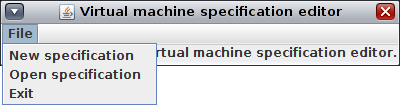
\includegraphics[scale=0.9]{assets/png/implemetation_gui_menu.png}
    \label{image:implemetation:gui:menu}
\end{figure}
Implementované grafické rozhraní využívá grafické knihovny Swing, která je podporována pouze na platformě JVM. Z~důvodů uvedených
v~kapitole \ref{chapter:implementation:language:ruby} je použití grafického rozhraní podmíněno využitím interpretu JRuby.
V~případě, že uživatel spustí grafické rozhraní na jiné platformě, aplikace se ukončí a~grafické rozhraní se nezobrazí. Ostatní
funkce nástroje nejsou závislé na použitém interpretu.
\subsection{Editor šablon}
\label{chapter:implementation:gui:editor}
Prvním využitím grafického rozhraní je editor pro manipulaci se šablonami zón. Tento editor se spouští pomocí příkazu \verb|editor|,
který je součástí uživatelského rozhraní klientské aplikace. Po spuštění tohoto příkazu je uživateli zobrazeno grafické okno,
které slouží pro editaci šablon.
\begin{figure}[t]
    \centering    
    \caption{Formulář editoru šablon}
    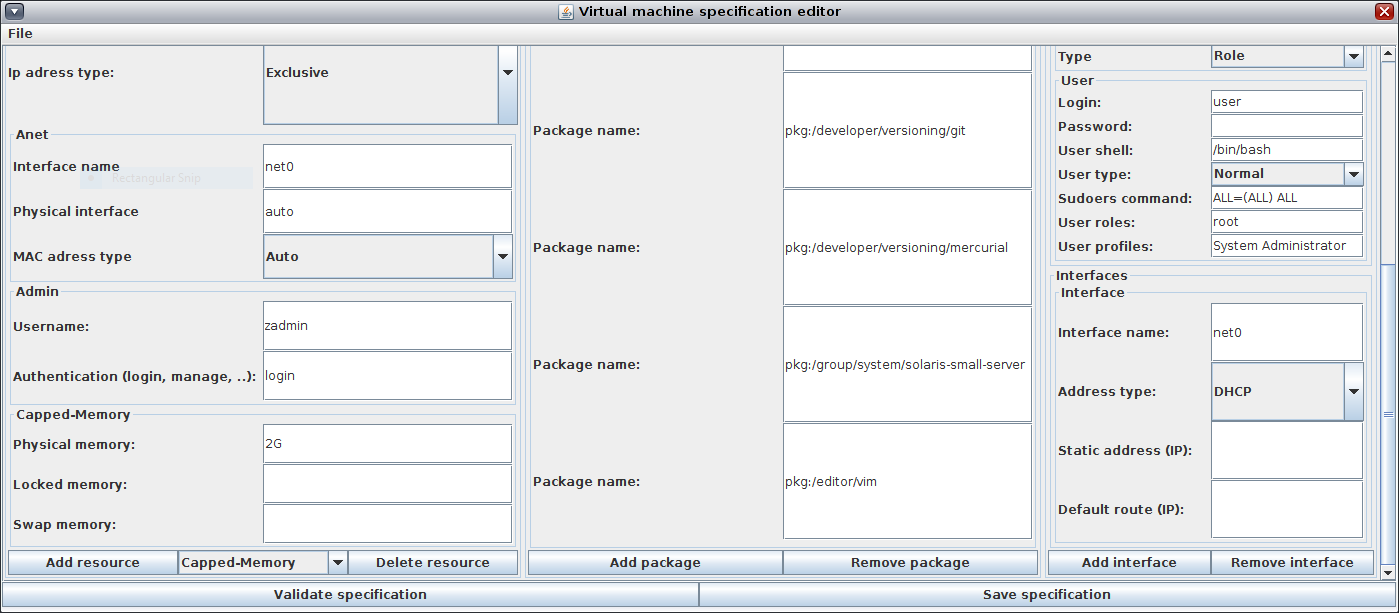
\includegraphics[scale=0.35]{assets/png/implemetation_gui_form.png}
    \label{image:implemetation:gui:form}
\end{figure}
Horní část editoru obsahuje ovládací panel, který umožňuje uživateli načítat šablony nebo vytvářet nové. Součástí tohoto panelu
je také tlačítko pro~ukončení editoru. Pokud uživatel zvolí možnost načtení šablony, je pomocí několika dialogových oken dotázán
na cestu k~dané šabloně. Po úspěšném zadání cesty se uživateli v~prostřední části editoru zobrazí formulář vyplněný pomocí
dat z~načtené šablony. Pokud uživatel vybere druhou možnost, kterou je vytvoření šablony, je v~prostřední části editoru zobrazen 
ten samý formulář, ale vyplněný implicitními hodnotami. Ovládací menu společně s~úvodním oknem editoru je zobrazeno na 
obrázku \ref{image:implemetation:gui:menu}.

Formulář pro vyplňování atributu šablony je umístěn ve středu editoru a~tvoří jeho nejpodstatnější část. Jelikož má struktura 
šablony neglobální zóny tři části, skládá se i hlavní okno editoru ze tří oddělených částí. Tyto části přímo odpovídají jednotlivým
sekcím šablony a~nazývají se konfigurace, manifest a~nastavení. Jak je patrné z obrázku \ref{image:implemetation:gui:form}, každá
sekce editoru má ve spodní části ovládací prvky. Tyto prvky slouží k~přidávání a~odebírání konfiguračních prvků ze šablony. Část s~konfigurací
umožňuje vybírat z~několika různých typů zdrojů, které lze v~editoru použít. V~druhé části editoru lze přidávat a~odebírat
softwarové balíky, které mají být v~instancích dané šablony nainstalované. Poslední část umožňuje přidávat a~odebírat nastavení
pro definované síťové adaptéry.

Poslední částí editoru je spodní ovládací panel, který obsahuje dvě funkční tlačítka. V~případě použití prvního tlačítka
pro validaci se pomocí knihovny vyvolá příslušná funkce a~šablona se ověří. Uživatel je o~výsledku informován pomocí dialogového
okna. Druhé tlačítko slouží k~uložení šablony do souboru a~uživatel je vyzván k~zadání jména šablony a~adresáře, kam se šablona má uložit.
V~obou případech dojde k~rekonstrukci datového formátu JSON popsaného v~kapitole \ref{chapter:implementation:szones:template},
který je vyplněn pomocí hodnot specifikovaných uživatelem v~editoru. Tato konstrukce šablon je pro uživatele jednodušší, protože
vždy vygeneruje validní šablonu. V~případě manuální tvorby musí uživatel zajistit její validitu.
\subsection{Interaktivní instalace}
\label{chapter:implementation:gui:interactive}
Grafické rozhraní je v~nástroji využito ještě v~případě, že uživatel spustí příkaz \verb|deploy| s~parametrem \textit{interactive}.
V~tomto případě je spuštěna interaktivní instalace a~uživateli je opět zobrazeno grafické okno. Toto okno je stejného charakteru
jako výše popsaný editor a~slouží ke specifikaci vlastností vytvářených zón. Uživatel nyní nebude mít na výběr z~načtení šablon, ale bude muset
zadat hodnoty manuálně. Některé atributy jsou vyplněny implicitními hodnotami a~uživatel musí zadat minimálně počáteční heslo 
uživatele \textit{root} a~konfiguraci počátečního systémového uživatele.
\section{Instalační balík}
\label{chapter:implementation:package}
Gem je standardní strukturou pro snadnou distribuci aplikací vyvíjených v programovacím jazyce Ruby. Tato struktura umožňuje vývojářům
jednoduše popsat vyvíjenou aplikaci nebo stanovit seznam závislostí, které jsou v průběhu instalace gemu vyřešeny. Instalace gemu
velice snadná a provádí se pomocí následujícího příkazu \mintinline{Ruby}{gem install packagename.gem}.

Všechny soubory a zdrojové kódy aplikace byly zabaleny do kompaktního instalačního balíčku \textit{szmgmt-1.0.0.gem}, který
slouží pro jednoduchou a rychlou instalaci celé aplikace.  Součástí tohoto balíčku jsou i spustitelné soubory \textit{szmgmt-cli} a
\textit{szmgmt-editor}, které slouží pro ovládání nástroje pro podporu automatické správy virtualizačního kontejneru Solaris Zones.
Postup instalace nástroje je popsaný v příloze \ref{appendix:installation} a instalační balík je společně se všemi zdrojovými kódy
nástroje dostupný z online repoziřáře \cite{tool:repository} nebo na přiloženém médiu.